
\paragraph{Khatri-Rao 积}
Khatri-Rao 积是按列进行的 Kronecker 积~\citep{smilde2005multi,bro1998multi}。设 $\Ab\in\RR^{m\times R}$ 且 $\Bb\in\RR^{n\times R}$。$\Ab$ 与 $\Bb$ 的 Khatri-Rao 积记为 $\Ab\krao\Bb\in\RR^{mn\times R}$，定义为
\begin{align*}
    \def\baseline{-0.5ex}
    \Ab\krao\Bb =
    \begin{bmatrix}
    \vline & \vline  &   & \vline \\
    \ab_1\kron\bb_1 & \ab_2\kron\bb_2 & \dots & \ab_R\kron\bb_R\\
    \vline & \vline & & \vline 
    \end{bmatrix}
=
    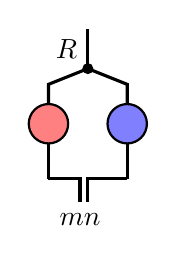
\begin{tikzpicture}[baseline=\baseline]
    \tikzset{tensor/.style = {minimum size = 0.5cm,shape = circle,thick,draw=black,inner sep = 0pt}, edge/.style   = {thick,line width=.4mm},every loop/.style={}}
    \def\y{0}
    \def\x{0}
    \node[tensor,fill=red!50!white] (A) at (\x,\y){$\Ab$};
    \node[tensor,fill=blue!50!white] (B) at (\x+1,\y){$\Bb$};
    \draw[edge] (\x,\y+0.25) -- (\x,\y+0.5) -- (\x+0.5,\y+0.7);
    \draw[edge] (\x+1,\y+0.25) -- (\x+1,\y+0.5) -- (\x+0.5,\y+0.7);
    \draw[edge] (\x+0.5,\y+0.7) -- (\x+0.5,\y+1.2) node [left, midway] {\edgelabel{$R$}};
    \draw  node[fill = black,circle,inner sep=0pt,minimum size=4pt] (m) at (\x+0.5,\y+0.7) {};
    \draw[edge] (\x,\y-0.25) -- (\x,\y-0.7);
    \draw[edge] (\x+1,\y-0.25) -- (\x+1,\y-0.7);
    \draw[edge] (\x+1,\y-0.7) -- (\x+0.5,\y-0.7) -- (\x+0.5,\y-1);
    \draw[edge] (\x+1,\y-0.25) -- (\x+1,\y-0.7);
    \draw[edge] (\x,\y-0.7) -- (\x+0.4,\y-0.7) -- (\x+0.4,\y-1)node [below] {\edgelabel{$mn$}};
    \end{tikzpicture}\hspace{0.5cm},
\end{align*}
其中 $\ab_1,\dots,\ab_R\in\RR^{m}$ 为 $\Ab$ 的各列，$\bb_1,\dots,\bb_R\in\RR^{n}$ 为 $\Bb$ 的各列。  在对应的张量网络图中，复制张量强制所得矩阵只包含 $\Ab$ 与 $\Bb$ 中\emph{相互匹配}的各列的 Kronecker 积。 
\begin{remark}
Khatri-Rao 积的部分性质列举如下：
\begin{enumerate}
\item 与 Kronecker 积类似，Khatri-Rao 积不满足交换律，即一般情况下 $\Ab\krao\Bb\neq \Bb\krao\Ab$。
\item Khatri-Rao 积满足结合律，即 $\Ab\krao(\Bb\krao\Cb)=(\Ab\krao\Bb)\krao\Cb$，其中 $\Ab\in\RR^{m\times R},\Bb\in\RR^{n\times R}$ 且 $\Cb\in\RR^{s\times R}$。
\item $\Ab\krao\Bb$ 的各列构成 Kronecker 积 $\Ab\kron \Bb$ 各列的一个子集。
\end{enumerate}
\end{remark}

\paragraph{Hadamard 积}
设 $\Ab\in\RR^{m\times n}$ 与 $\Bb\in\RR^{m\times n}$ 为形状相同的矩阵。$\Ab$ 与 $\Bb$ 的 Hadamard 积（或称逐分量积）是矩阵  $\Ab\hadam\Bb\in\RR^{m\times n}$，按元素定义为 
$$(\Ab\hadam\Bb)_{ij} = \Ab_{ij}\Bb_{ij}.$$
在张量网络图中，Hadamard 积可以很方便地用复制张量表示：
\begin{equation*}
\Ab\hadam\Bb =
     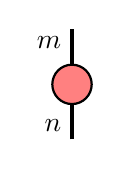
\begin{tikzpicture}[baseline=\baseline]
    \tikzset{tensor/.style = {minimum size = 0.5cm,shape = circle,thick,draw=black,inner sep = 0pt}, edge/.style   = {thick,line width=.4mm},every loop/.style={}}
    \def\y{0}
    \def\x{0}
    \draw[edge] (\x,\y-0.7) -- (\x,\y+0.7)  node [very near end,left] {\edgelabel{$m$}} node [very near start,left] {\edgelabel{$n$}} ;
    \node[tensor,fill=red!50!white] (A) at (\x,\y){$\Ab$};
    \end{tikzpicture} 
    \ \hadam %
    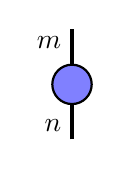
\begin{tikzpicture}[baseline=\baseline]
    \tikzset{tensor/.style = {minimum size = 0.5cm,shape = circle,thick,draw=black,inner sep = 0pt}, edge/.style   = {thick,line width=.4mm},every loop/.style={}}
    \def\y{0}
    \def\x{0}
    \draw[edge] (\x,\y-0.7) -- (\x,\y+0.7)node [very near end,left] {\edgelabel{$m$}} node [very near start,left] {\edgelabel{$n$}} ;
    \node[tensor,fill=blue!50!white] (B) at (\x,\y){$\Bb$};
    \end{tikzpicture}
\ =
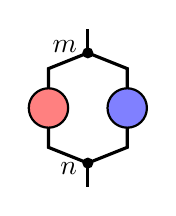
\begin{tikzpicture}[baseline=\baseline]
    \tikzset{tensor/.style = {minimum size = 0.5cm,shape = circle,thick,draw=black,inner sep = 0pt}, edge/.style   = {thick,line width=.4mm},every loop/.style={}}
    \def\y{0}
    \def\x{0}
    \node[tensor,fill=red!50!white] (A) at (\x,\y){$\Ab$};
    \node[tensor,fill=blue!50!white] (B) at (\x+1,\y){$\Bb$};
    \draw[edge] (\x,\y+0.25) -- (\x,\y+0.5) -- (\x+0.5,\y+0.7);
    \draw[edge] (\x+1,\y+0.25) -- (\x+1,\y+0.5) -- (\x+0.5,\y+0.7);
    \draw[edge] (\x+0.5,\y+0.7) -- (\x+0.5,\y+1) node [near start,left] {\edgelabel{$m$}};
    \draw  node[fill = black,circle,inner sep=0pt,minimum size=4pt] (m) at (\x+0.5,\y+0.7) {};
    \draw[edge] (\x,\y-0.25) -- (\x,\y-0.5) -- (\x+0.5,\y-0.7);
    \draw[edge] (\x+1,\y-0.25) -- (\x+1,\y-0.5) -- (\x+0.5,\y-0.7);
    \draw[edge] (\x+0.5,\y-0.7) -- (\x+0.5,\y-1) node [near start,left] {\edgelabel{$n$}};
    \draw  node[fill = black,circle,inner sep=0pt,minimum size=4pt] (m) at (\x+0.5,\y-0.7) {};
\end{tikzpicture}.
\end{equation*}
更一般地，对任意 $\Ab_1\in\RR^{m\times n},\dots,\Ab_d\in\RR^{m\times n}$，有 
\begin{align*}
\Ab_1\hadam\Ab_2\dots\hadam\Ab_{d} 
=
    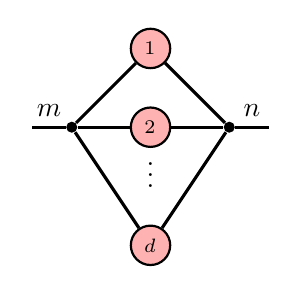
\begin{tikzpicture}[baseline=\baseline]
    \tikzset{tensor/.style = {minimum size = 0.5cm,shape = circle,thick,draw=black,inner sep = 0pt}, edge/.style   = {thick,line width=.4mm},every loop/.style={}}
    \def\y{1}
    \def\x{0}
    \node[tensor,fill=red!30!white] (A_1) at (\x,\y){$\Ab_1$};
    \node[tensor,fill=red!30!white] (A_2) at (\x,\y-1){$\Ab_2$};
    \node[draw=none] at (\x,\y-1.5) {\scalebox{1}{\textcolor{black}{$\vdots$}}};
    \node[tensor,fill=red!30!white] (A_N) at (\x,\y-2.5){$\Ab_d$};
    \draw  node[fill = black,circle,inner sep=0pt,minimum size=4pt] (m) at (\x+1,\y-1) {};
    \draw  node[fill = black,circle,inner sep=0pt,minimum size=4pt] (n) at (\x-1,\y-1) {};
    \draw[edge] (A_1) -- (m);
    \draw[edge] (A_2) -- (m);
    \draw[edge] (A_N) -- (m);
    \draw[edge] (A_1) -- (n);
    \draw[edge] (A_2) -- (n);
    \draw[edge] (A_N) -- (n);
    \draw[edge] (m) -- (\x+1.5,\y-1)node [midway,above] {\edgelabel{$n$}};
    \draw[edge] (n) -- (\x-1.5,\y-1)node [midway,above] {\edgelabel{$m$}};
    \end{tikzpicture}.
\end{align*}
\begin{remark}
这里列出 Hadamard 积的若干有用性质。
\begin{itemize}
    \item 元素取值于 $\{0,1\}$ 的张量 $\Tt$ 与自身的 Hadamard 积仍是 $\Tt$。特别地，这对复制张量成立：
    
    设 $\Tt\in\RR^{d_1\times d_2\times d_3}$ 为一个三阶复制张量。则在张量网络中，Hadamard 积 $\Tt\hadam\Tt$ 为：
    $$\Tt\hadam\Tt=
    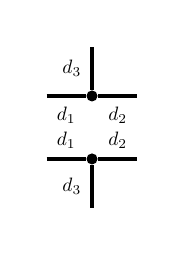
\begin{tikzpicture}[baseline=\baseline]
   \tikzset{tensor/.style = {minimum size = 0.5cm,shape = circle,thick,draw=black,inner sep = 0pt}, edge/.style = {thick,line width=.4mm},every loop/.style={}}
    \def\y{0.2}
    \def\x{0}
     \draw  node[fill = black,circle,inner sep=0pt,minimum size=4pt] (m) at (\x,\y-0.5) {};
     \draw  node[draw=none] (a) at (\x-0.7,\y-0.5) {};
     \draw  node[draw=none] (b) at (\x+0.7,\y-0.5) {};
     \draw  node[draw=none] (c) at (\x,\y-1.25) {};
    \draw[edge] (a) -- (m) node [midway,above] {\scalebox{0.7}{\dimcolor{$d_1$}}};
    \draw[edge] (m) -- (b)node [midway,above] {\scalebox{0.7}{\dimcolor{$d_2$}}};
    \draw[edge] (m) -- (c)node [midway,left] {\scalebox{0.7}{\dimcolor{$d_3$}}};
    \draw  node[fill = black,circle,inner sep=0pt,minimum size=4pt] (m1) at (\x,\y+0.3) {};
     \draw  node[draw=none] (d) at (\x-0.7,\y+0.3) {};
     \draw  node[draw=none] (e) at (\x+0.7,\y+0.3) {};
     \draw  node[draw=none] (f) at (\x,\y+1.05) {};
    \draw[edge] (d) -- (m1)node [midway,below] {\scalebox{0.7}{\dimcolor{$d_1$}}};
    \draw[edge] (m1) -- (e)node [midway,below] {\scalebox{0.7}{\dimcolor{$d_2$}}};
    \draw[edge] (m1) -- (f)node [midway,left] {\scalebox{0.7}{\dimcolor{$d_3$}}};
    \node[draw=none] at (\x,\y-0.15){$\hadam$};
\end{tikzpicture}
=
    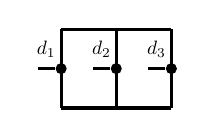
\begin{tikzpicture}[baseline=\baseline]
   \tikzset{tensor/.style = {minimum size = 0.5cm,shape = circle,thick,draw=black,inner sep = 0pt}, edge/.style = {thick,line width=.4mm},every loop/.style={}}
    \def\y{0}
    \def\x{0}
    \draw[edge](\x-0.7,\y-0.5)--(\x+0.7,\y-0.5);
    \draw[edge](\x-0.7,\y+0.5)--(\x+0.7,\y+0.5);
    \draw[edge](\x-0.7,\y-0.5)--(\x-0.7,\y+0.5);
    \draw[edge](\x+0.7,\y-0.5)--(\x+0.7,\y+0.5);
    \draw[edge](\x,\y+0.5) -- (\x,\y-0.5);
     \draw  node[fill = black,circle,inner sep=0pt,minimum size=4pt] (m1) at (\x-0.7,\y) {};
    \draw  node[fill = black,circle,inner sep=0pt,minimum size=4pt] (m) at (\x,\y) {};
    \draw  node[fill = black,circle,inner sep=0pt,minimum size=4pt] (m2) at (\x+0.7,\y) {};
    \draw[edge](m1)--(\x-1,\y)node [midway,above] {\scalebox{0.7}{\dimcolor{$d_1$}}};
    \draw[edge](m2)--(\x+0.4,\y)node [midway,above] {\scalebox{0.7}{\dimcolor{$d_3$}}};
    \draw[edge](m)--(\x-0.3,\y)node [midway,above] {\scalebox{0.7}{\dimcolor{$d_2$}}};
     \end{tikzpicture}$$
    
